% Editable working manuscript in APS/REVTeX style.
% This is intentionally a model-paper draft, NOT a claim of a completed microscopic
% finite-q ultrasonic calculation. See README.md in this directory for scope and figures.
% Compile from this directory with REVTeX 4.2 and the APS bibliography style installed.
\documentclass[aps,prb,preprint,superscriptaddress]{revtex4-2}

\usepackage{amsmath,amssymb,bm,graphicx}
\usepackage[colorlinks=true,citecolor=blue,linkcolor=blue,urlcolor=blue]{hyperref}
\graphicspath{{../../ultrasonic/figures/}{../../ultrasonic/figures/strict_policy/}{../../ultrasonic/analysis/wwn_temperature_maxima/}}

\newcommand{\kb}{k_{\mathrm B}}
\newcommand{\hbarw}{\hbar\omega}
\newcommand{\Dbar}{\bar\Delta}
\newcommand{\Emin}{E_{\min}}
\newcommand{\Wsc}{W_{\mathrm{sc}}}
\newcommand{\WN}{W_{\mathrm N}}
\newcommand{\Rsc}{R_{\mathrm{sc}}}

\begin{document}

\title{Quasiparticle absorption in a Rashba-correlated-hopping superconductor: a constant-vertex model and its limits}

\author{Reza Afzali}
\author{Bahman Takrim}
\author{Amir Hossein Asghari}
\affiliation{Department of Physics, K. N. Toosi University of Technology, Tehran 15875-4416, Iran}

\date{\today}

\begin{abstract}
We re-examine the finite-frequency quasiparticle-scattering contribution to the normalized absorption of a square-lattice superconducting model with correlated hopping and Rashba spin-orbit coupling. Starting from the helicity-resolved quasiparticle spectrum, we retain the signed band-energy dependence of the gap and derive the Case-I Bogoliubov coherence factor and the two-root quasiparticle density of states. The resulting energy-space integral conserves quasiparticle energy and uses a normal-state reference computed from the same lattice density of states. We also identify a limitation that prevents interpreting the existing curves as a microscopic ultrasonic-attenuation prediction: the electronic Hamiltonian does not specify its strain derivatives, while the implemented transition kernel replaces a momentum-resolved acoustic vertex by a constant matrix element and unrestricted initial-to-final momentum sums. We therefore report the numerical curves only as results of this phenomenological constant-vertex model. The acoustic coupling, finite-wave-vector response, screening, and disorder corrections remain material-dependent and unresolved.
\end{abstract}

\maketitle

\section{Introduction}

Absorption by a superconductor probes the allowed transitions between Bogoliubov quasiparticles and the coherence factors associated with those transitions. In noncentrosymmetric systems, Rashba spin-orbit coupling (SOC) also changes the normal-state bands and can alter the superconducting spectrum. These ingredients motivate studying absorption in correlated lattice models with SOC.

The electronic model used here is based on the square-lattice Hubbard model with correlated hopping and Rashba coupling of Hutchinson, Hirsch, and Marsiglio (HHM)~\cite{HHM}. HHM determines an electronic pairing problem; it does not, by itself, give an electron--ion coupling. In particular, an acoustic displacement can modulate the on-site potential, ordinary hopping, correlated hopping, and Rashba interaction. The corresponding derivatives with respect to strain are not fixed by the equilibrium electronic Hamiltonian.

The original manuscript associated with this project treated the transition matrix element as a constant after angular and spin averaging. This provides a phenomenological energy-integrated model, but it is not equivalent in general to a clean acoustic phonon with fixed wave vector. We make that distinction explicit. The present paper derives and documents the constant-matrix-element quasiparticle-scattering calculation, corrects its coherence factor and energy-space measure, and uses the existing calculations as conditional model results. It does not claim that the available data determine the physical finite-$q$ ultrasonic response of a particular material.

\section{Electronic model and quasiparticle spectrum}

We work in units $t=\hbar=\kb=1$ unless stated otherwise. The normal-state helicity bands are
\begin{align}
 \epsilon_{\bm k s} &= \epsilon_{\bm k}^{(0)}-2sV_{\mathrm{SO}}R_{\bm k},\qquad s=\pm1,\\
 \epsilon_{\bm k}^{(0)}&=-2t(\cos k_x+\cos k_y),\\
 R_{\bm k}&=\sqrt{\sin^2 k_x+\sin^2 k_y}.
\end{align}
Here $s$ labels Rashba helicity. It is distinct from the index $\sigma=\pm1$ used below to label the two roots of the quasiparticle-energy inversion.

Within the HHM mean-field solution used by the production calculations, the real gap amplitude is linear in the helicity-band energy,
\begin{equation}
 \Dbar(\epsilon)=D_0-b\epsilon,\qquad b=\frac{D_S}{4t},
\end{equation}
so that
\begin{equation}
 \xi=\epsilon-\mu,\qquad E(\epsilon)=\sqrt{\xi^2+\Dbar(\epsilon)^2}.
 \label{eq:qpenergy}
\end{equation}
The calculation assumes the HHM intraband, time-reversed pairing structure and uses the corresponding real, even gap amplitude. It does not solve a general multicomponent order parameter.

Completing the square gives
\begin{align}
 E^2(\epsilon)&=\kappa^2(\epsilon-\epsilon_*)^2+\Emin^2,\\
 \kappa&=\sqrt{1+b^2},\qquad
 \epsilon_* = \frac{\mu+bD_0}{1+b^2},\qquad
 \Emin=\frac{|D_0-b\mu|}{\kappa}.
 \label{eq:complete-square}
\end{align}
For every $E\geq\Emin$, there are up to two band-energy roots,
\begin{equation}
 \ell=\sqrt{E^2-\Emin^2},\qquad
 \epsilon_\sigma(E)=\epsilon_*+\sigma\frac{\ell}{\kappa},\qquad
 \xi_\sigma=\epsilon_\sigma-\mu,\qquad
 \Dbar_\sigma=D_0-b\epsilon_\sigma.
 \label{eq:branches}
\end{equation}
The roots are retained only where $\epsilon_\sigma$ lies within the exact support of the chosen lattice band. We use $\sigma$ for the branch label and reserve $s$ for helicity.

Let $N(\epsilon)=\sum_sN_s(\epsilon)$ be the normal-state density of states (DOS) summed over both helicity bands in the normalization used by the code. The branch-resolved quasiparticle DOS is
\begin{equation}
 \nu_\sigma(E)=N\!\left(\epsilon_\sigma(E)\right)
 \left|\frac{d\epsilon_\sigma}{dE}\right|
 =N\!\left(\epsilon_\sigma(E)\right)\frac{E}{\kappa\ell}.
 \label{eq:qpDOS}
\end{equation}
The Jacobian is exact for Eq.~(\ref{eq:qpenergy}); its edge singularity is integrable and is removed from the numerical quadrature by changing variables from $E$ to $\ell$.

\section{Acoustic vertex: what is and is not specified}

A general linear strain coupling has the form
\begin{equation}
 \delta H_{\mathrm{ep}}=\sum_{ab}\frac{\partial H_{\mathrm{HHM}}}{\partial\epsilon_{ab}}\,\epsilon_{ab},\qquad
 \epsilon_{ab}=\frac12(\partial_a u_b+\partial_b u_a).
 \label{eq:strain}
\end{equation}
The derivative may contain deformation-potential, hopping, correlated-hopping, and SOC terms. For example, a scalar deformation potential contributes $D_{ab}\epsilon_{ab}n$, whereas a bond-length-dependent hopping produces a momentum- and bond-direction-dependent vertex. A strain-dependent Rashba interaction produces a spin-matrix vertex. Their strengths require microscopic derivatives such as $\partial t/\partial\epsilon_{ab}$, $\partial D_t/\partial\epsilon_{ab}$, and $\partial V_{\mathrm{SO}}/\partial\epsilon_{ab}$, as well as phonon eigenvectors and normalization. These inputs are not specified in the HHM Hamiltonian or in the numerical parameter files.

The implemented model instead uses an effective spin-independent constant matrix element $B$ and a density-like operator,
\begin{equation}
 H'(t)=B\sum_{\bm q}(b_{\bm q}+b^\dagger_{-\bm q})\rho_{\bm q},\qquad
 \rho_{\bm q}=\sum_{\bm k s}c^\dagger_{\bm{k+q},s}c_{\bm k s}.
 \label{eq:phenom-vertex}
\end{equation}
The constant $B$ is treated as independent of $\bm k$, $\bm q$, helicity, and phonon polarization. It is not calculated from Eq.~(\ref{eq:strain}). In the reported ratio, its prefactor cancels only under this shared-constant-vertex assumption.

For a scalar spin-independent vertex, the Rashba-helicity overlap at finite $q$ is
\begin{equation}
 \left|\langle u_{s',\bm{k+q}}|u_{s,\bm k}\rangle\right|^2
 =\frac{1+ss'\widehat{\bm g}_{\bm{k+q}}\cdot\widehat{\bm g}_{\bm k}}{2},
 \label{eq:helicity-overlap}
\end{equation}
where $\bm g_{\bm k}$ is the Rashba spin-orbit field. At $q=0$ and away from helicity degeneracies, this overlap is helicity diagonal. The standard production DOS convolution does not retain this selection: the product of total DOS factors includes all helicity-pair combinations with equal vertex weight. A separate same-helicity diagnostic exists, but it still does not impose fixed-$q$ momentum conservation.

For an actual clean phonon calculation, crystal momentum would obey $\bm k'=\bm k+\bm q+\bm G$, with reciprocal vector $\bm G$, and the phonon energy would satisfy $\omega_{\bm q\lambda}=v_{s,\lambda}|\bm q|$ in the long-wavelength isotropic limit. In a BdG/Nambu calculation with eigenvectors $|\Phi_{m\bm k}\rangle$, the matrix element would be
\begin{equation}
 M_{nm}(\bm k,\bm q,\lambda)=
 \langle\Phi_{n,\bm{k+q}}|\Gamma_{\bm q\lambda}(\bm k)|\Phi_{m\bm k}\rangle,
 \label{eq:bdg-matrix-element}
\end{equation}
where $\Gamma$ is the Nambu lift of the specified microscopic electron--phonon vertex. The actual acoustic branch, $v_s$, polarization, screening, and microscopic vertex are not available, so Eq.~(\ref{eq:bdg-matrix-element}) is not evaluated numerically here.

\section{Scattering response in the constant-vertex model}

For the scalar Case-I process, the Bogoliubov scattering amplitude is $u u'-v v'$. With signed $\xi$ and signed gap amplitudes, its squared coherence factor is
\begin{equation}
 C_{\mathrm{I}}(E,\sigma;E',\sigma')
 =\frac12\left[1+\frac{\xi_\sigma(E)\xi_{\sigma'}(E')-
 \Dbar_\sigma(E)\Dbar_{\sigma'}(E')}{EE'}\right].
 \label{eq:coherence}
\end{equation}
This is the Case-I factor for the stated scalar vertex and mean-field Bogoliubov transformation. Replacing $\xi\xi'$ by $|\xi||\xi'|$, or changing the sign of the gap-product term, does not follow from that matrix element and is not used for the primary result.

Fermi's golden rule for absorption of one quantum of energy $\hbar\omega$ gives, up to the common mode and volume normalization,
\begin{align}
 \Wsc &\propto \frac{2\pi}{\hbar}(\hbar\omega)|B|^2 S_{\mathrm{sc}},\\
 S_{\mathrm{sc}}&=\sum_{\sigma,\sigma'}\int dE\,
 \nu_\sigma(E)\nu_{\sigma'}(E+\hbar\omega)
 C_{\mathrm I}(E,\sigma;E+\hbar\omega,\sigma')
 [f(E)-f(E+\hbar\omega)],
 \label{eq:scattering-integral}
\end{align}
with $f(E)=[e^{E/(\kb T)}+1]^{-1}$. The energy delta function has already been used to set $E'=E+\hbar\omega$. Each branch pair has its own band-support integration limits.

The normal reference is the $D_0=D_S=0$ limit of the same energy-averaged model,
\begin{equation}
 S_{\mathrm N}=\int d\epsilon\,N(\epsilon)N(\epsilon+\hbar\omega)
 [f_{\mathrm N}(\epsilon;\mu_{\mathrm N})-f_{\mathrm N}(\epsilon+\hbar\omega;\mu_{\mathrm N})],
 \qquad
 \Rsc=\frac{S_{\mathrm{sc}}}{S_{\mathrm N}}.
 \label{eq:ratio}
\end{equation}
Here $\mu_{\mathrm N}(T)$ is obtained from the normal-state number equation at the same filling. Equation~(\ref{eq:ratio}) is a ratio for the assumed constant-vertex model. If the physical vertex varies over the Fermi surface or helicity bands, it must be included in both numerator and denominator and need not cancel.

The same operator also has an anomalous pair-creation channel with $E+E'=\hbar\omega$, thermal factor $1-f(E)-f(E')$, and complementary coherence factor $C_{\mathrm p}=1-C_{\mathrm I}$ for this scalar mean-field vertex. Its kinematic threshold in this model is
\begin{equation}
 \hbar\omega>2\Emin(T),
 \label{eq:pair-threshold}
\end{equation}
not $2\Delta_{\mathrm{eff}}$ in general. The plotted principal quantity is $\Rsc$, the scattering component only. It is the complete modeled absorption only where Eq.~(\ref{eq:pair-threshold}) is not satisfied. We do not report a full finite-$q$ absorption ratio.

\section{Numerical procedure and parameter choices}

The master set uses $U/t=95$, $\Delta_t/t=4.5$, $n=1.885$, and $\hbar\omega/t=0.7$, with $t=\hbar=\kb=1$. Other panels show the parameter sets indicated in their captions. The stage-one nonlinear solver supplies $T_c,D_0(0),D_S(0)$; its operational $T_c$ is a nonlinear gap-threshold proxy and is not the HHM linearized-determinant criterion. At finite temperature, the project scales $D_0$ and $D_S$ with the common fitted shape
\begin{equation}
 \phi(T)=\left[1-(T/T_c)^{3.434}\right]^{0.553},
 \label{eq:gap-fit}
\end{equation}
for all SOC values, then solves the number equation for $\mu_{\mathrm{SC}}(T)$ and $\mu_{\mathrm N}(T)$ on finite midpoint grids. This rigid-shape fit is a modeling choice, not a finite-temperature self-consistent gap solution.

The normal-state DOS is sampled on a quarter-zone midpoint grid, histogrammed into 48,000 bins, Gaussian-smoothed with width $0.0025t$, normalized to total integral 2, and set to zero outside the exact band support. The production scattering integral uses the $\ell$ variable and a midpoint quadrature with 6,000 points per branch pair. The normal integral uses a kink-aligned Gauss--Legendre rule with an order-$n$ versus order-$(n+2)$ convergence check. The independent lattice cross-check bins energies, uses Gaussian broadening for the energy delta, and extrapolates in the broadening width; it validates the numerical energy reduction within the same unrestricted-transition model, not a finite-$q$ acoustic theory.

For parameter-family plots, we use the repository's strict bare-band chemical-potential policy as the primary displayed set. The strict-family figure provenance records stage-one $N_k=80$, stage-two chemical-potential $N_k=200$, DOS $N_k=1200$, and 20{,}000 energy-quadrature points per branch pair; these figure-specific resolutions differ from the default single-run values above. Missing roots or out-of-band stage-two points are omitted/gapped, not assigned zero. Relaxed-policy outputs are retained separately as diagnostics. The strict criterion establishes band admissibility only; it does not compare free energies between multiple in-band roots.

\section{Results: conditional model behavior}

The figures in this section report the energy-averaged, constant-vertex scattering ratio. Strict-window outputs are the primary admissibility results: a missing strict root or rejected stage-two state is shown as a gap, not as zero response. These curves remain conditional on the fitted gap inputs and the shared matrix element; they are not a material-specific finite-$q$ ultrasonic prediction.

\subsection{Strict-window parameter families}

The first three figures show complementary views of the strict-policy families. The $U$-scan resolves the sampled response across interaction strength at five fixed SOC values, while the SOC-scan shows the converse family at several fixed $U$. The temperature/gap panels retain the existing strict-window comparison to the supplied gap scale. The square markers in the $U$-scan denote the generator's $D_0(0)<0.05t$ diagnostic; they are not zero-response markers. The printed no-root counts and gaps identify where no strict superconducting root was accepted.

\begin{figure}[t]
 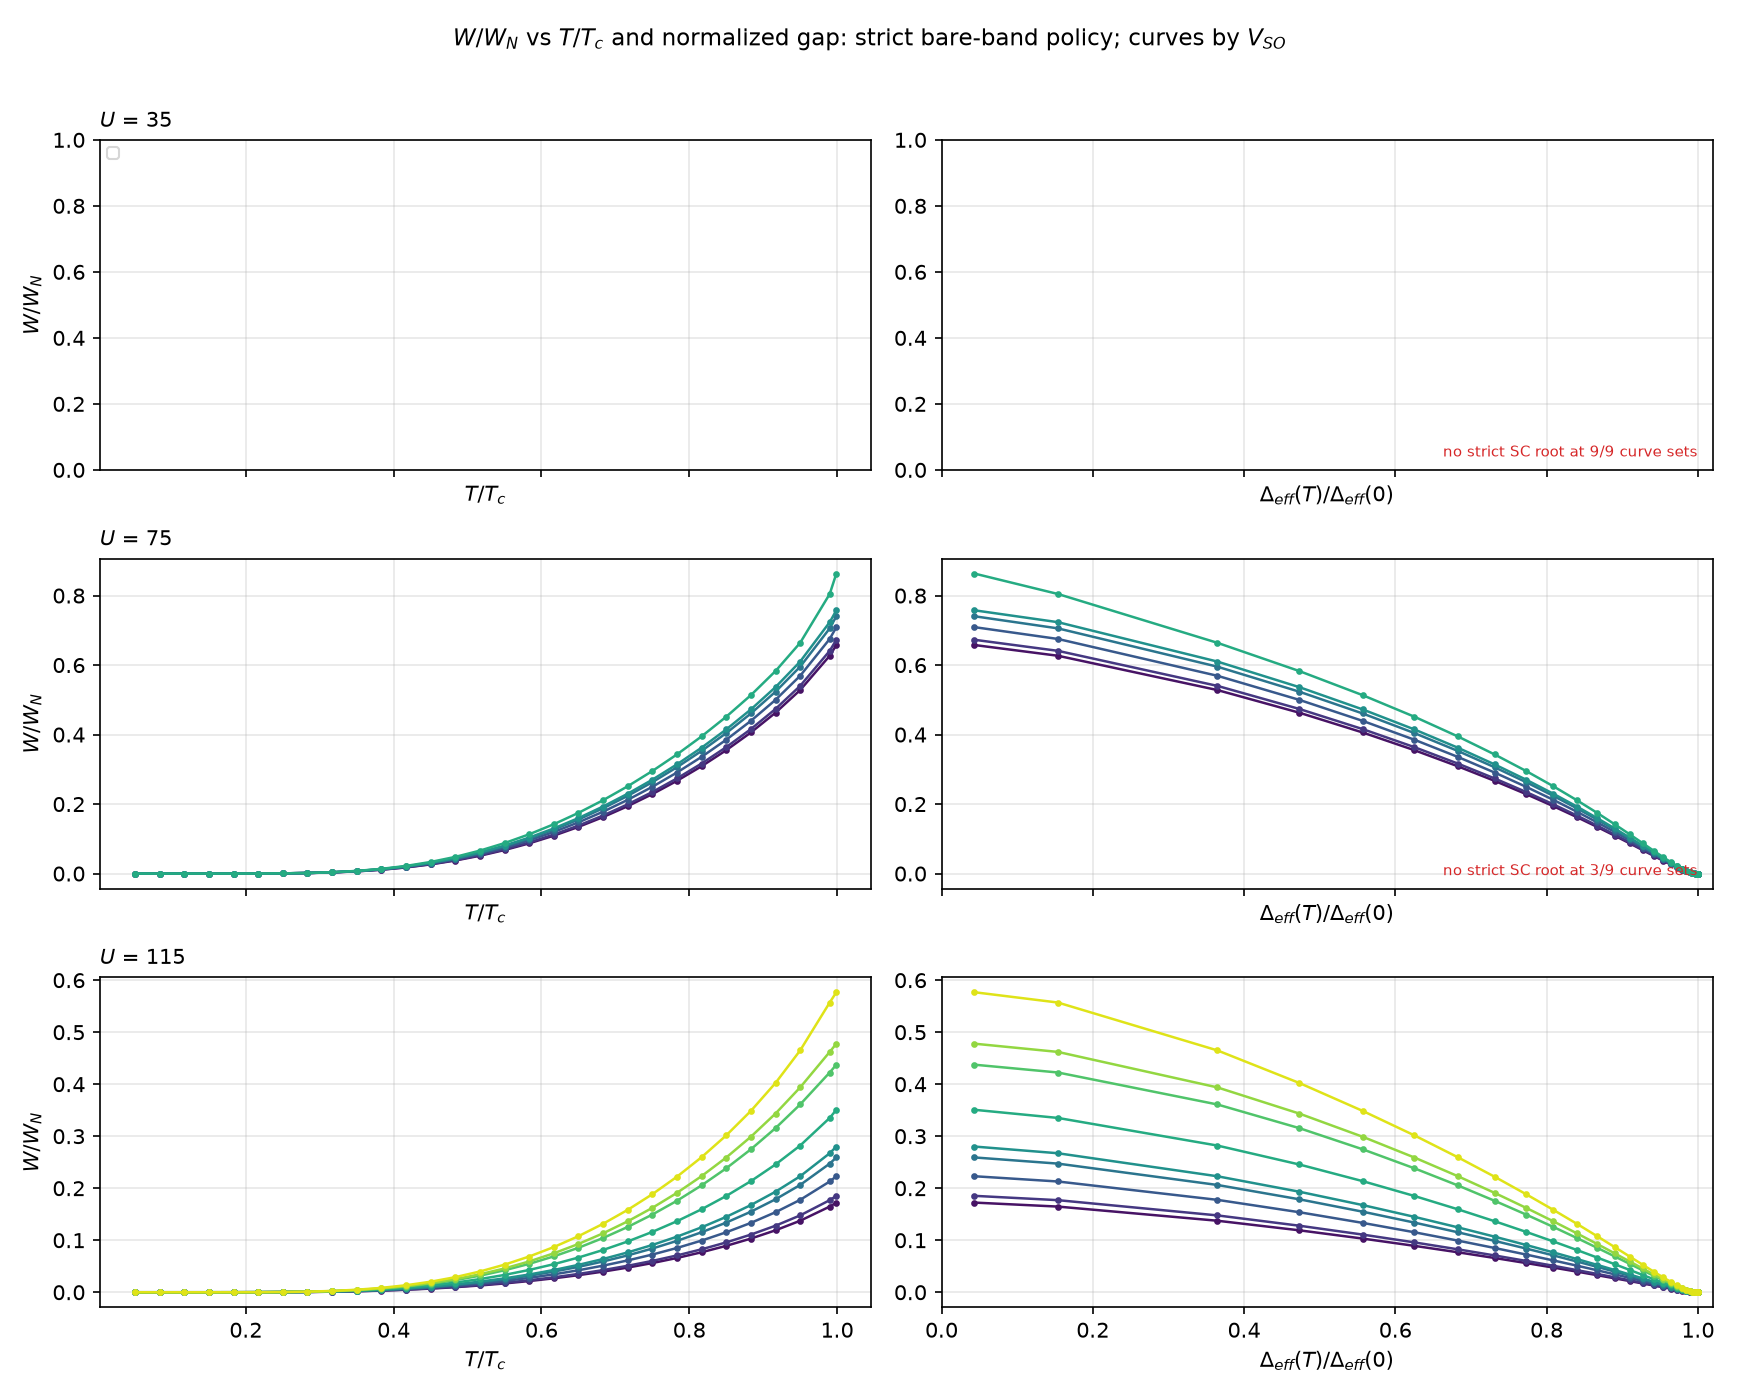
\includegraphics[width=\linewidth]{strict_policy/WWN_vs_TTc_and_Delta_VSOfamilies.png}
 \caption{Strict-window constant-vertex scattering ratio versus $T/T_c$ and normalized effective gap for the parameter families identified in the panels. Only strict band-admissible roots are displayed. Blank regions and gaps indicate absent or rejected samples, not zero absorption. These model results show the scattering channel only; they omit the finite-$q$ acoustic vertex and any pair-creation contribution above its threshold.}
 \label{fig:strict-temperature}
\end{figure}

\begin{figure}[t]
 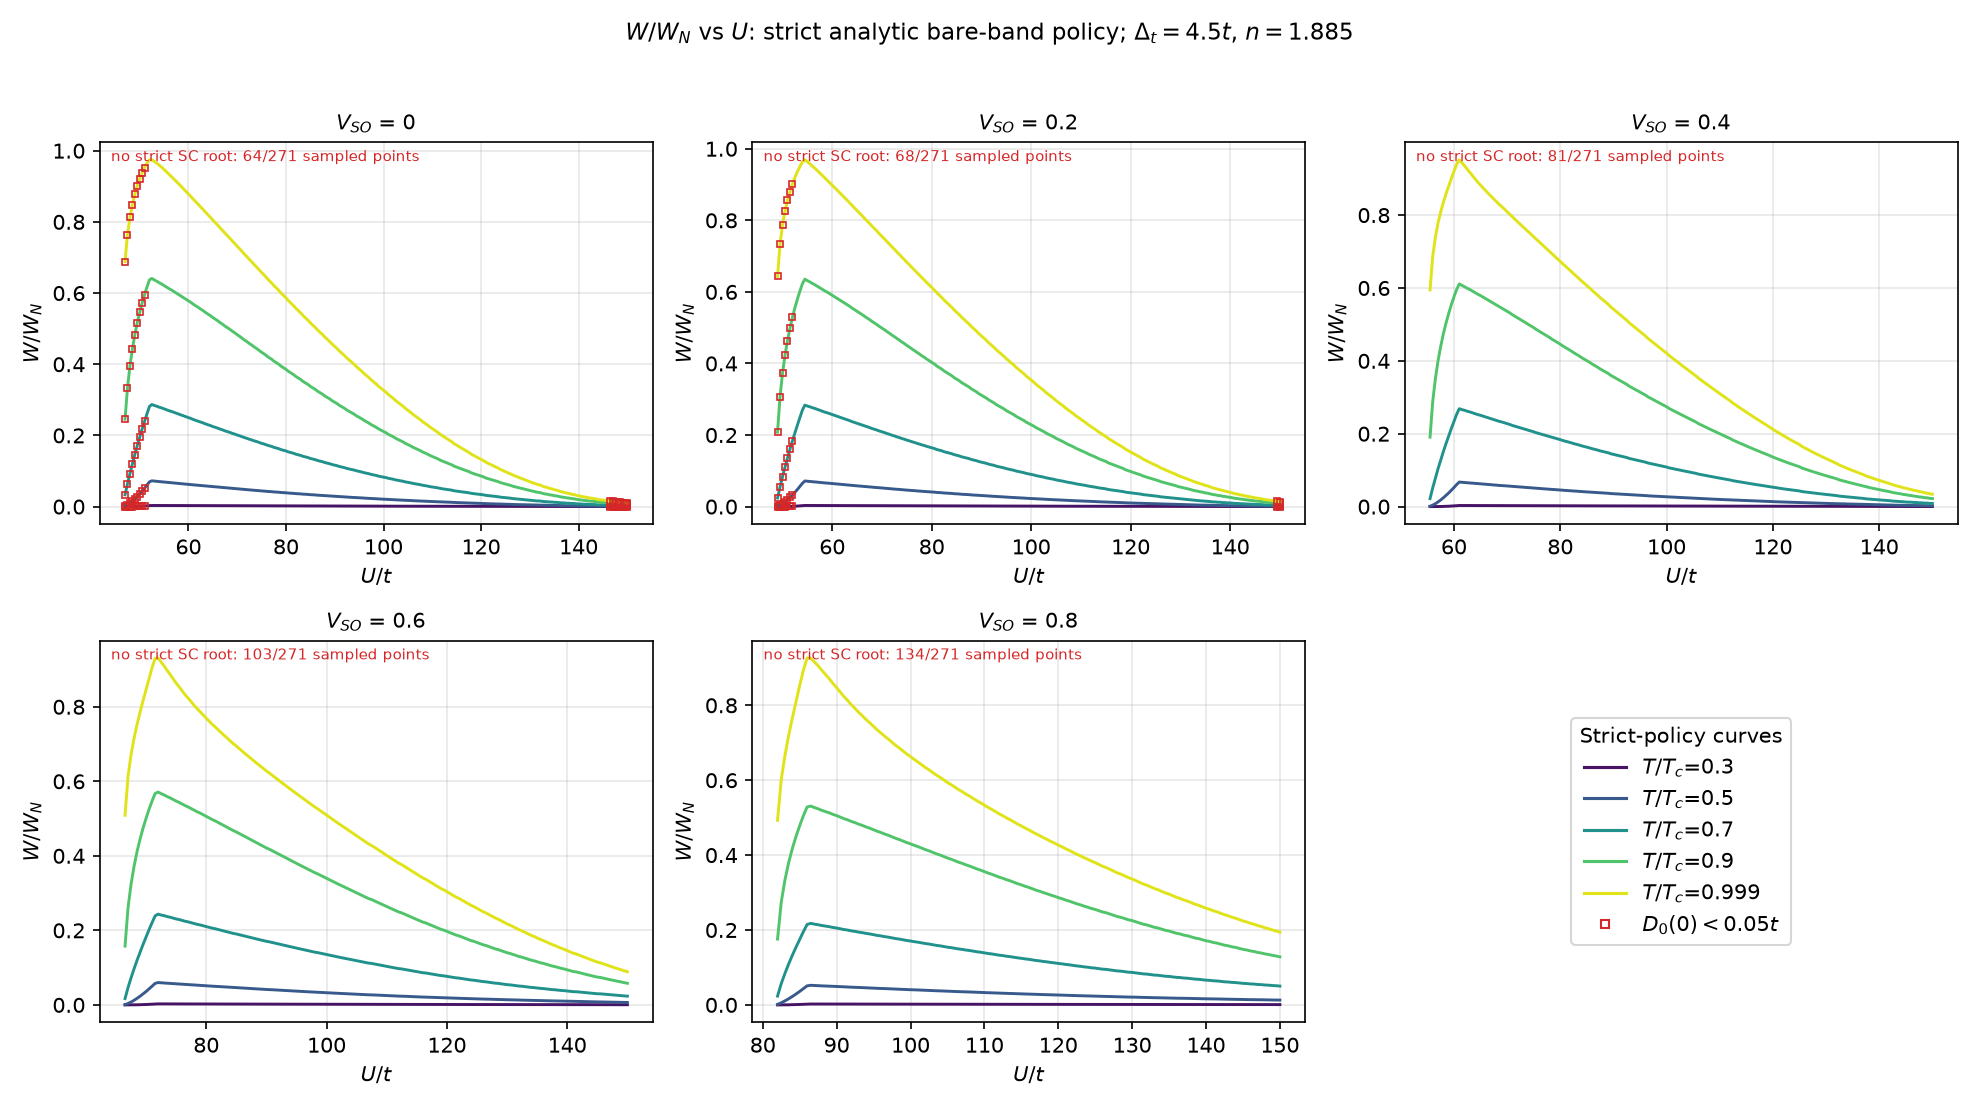
\includegraphics[width=\linewidth]{strict_policy/WWN_vs_U_families_VSO.png}
 \caption{Strict-window $W/W_N$ versus $U/t$ for the SOC families marked in the panels, with the sampled temperature fractions shown in the legend. Red open squares mark points with $D_0(0)<0.05t$ as defined by the figure generator; the red annotations give the number of sampled points without a strict superconducting root. Missing or rejected samples remain gaps rather than zeros. This is the primary strict-admissibility $U$-family result for the conditional constant-vertex scattering model.}
 \label{fig:strict-u-families}
\end{figure}

\begin{figure}[t]
 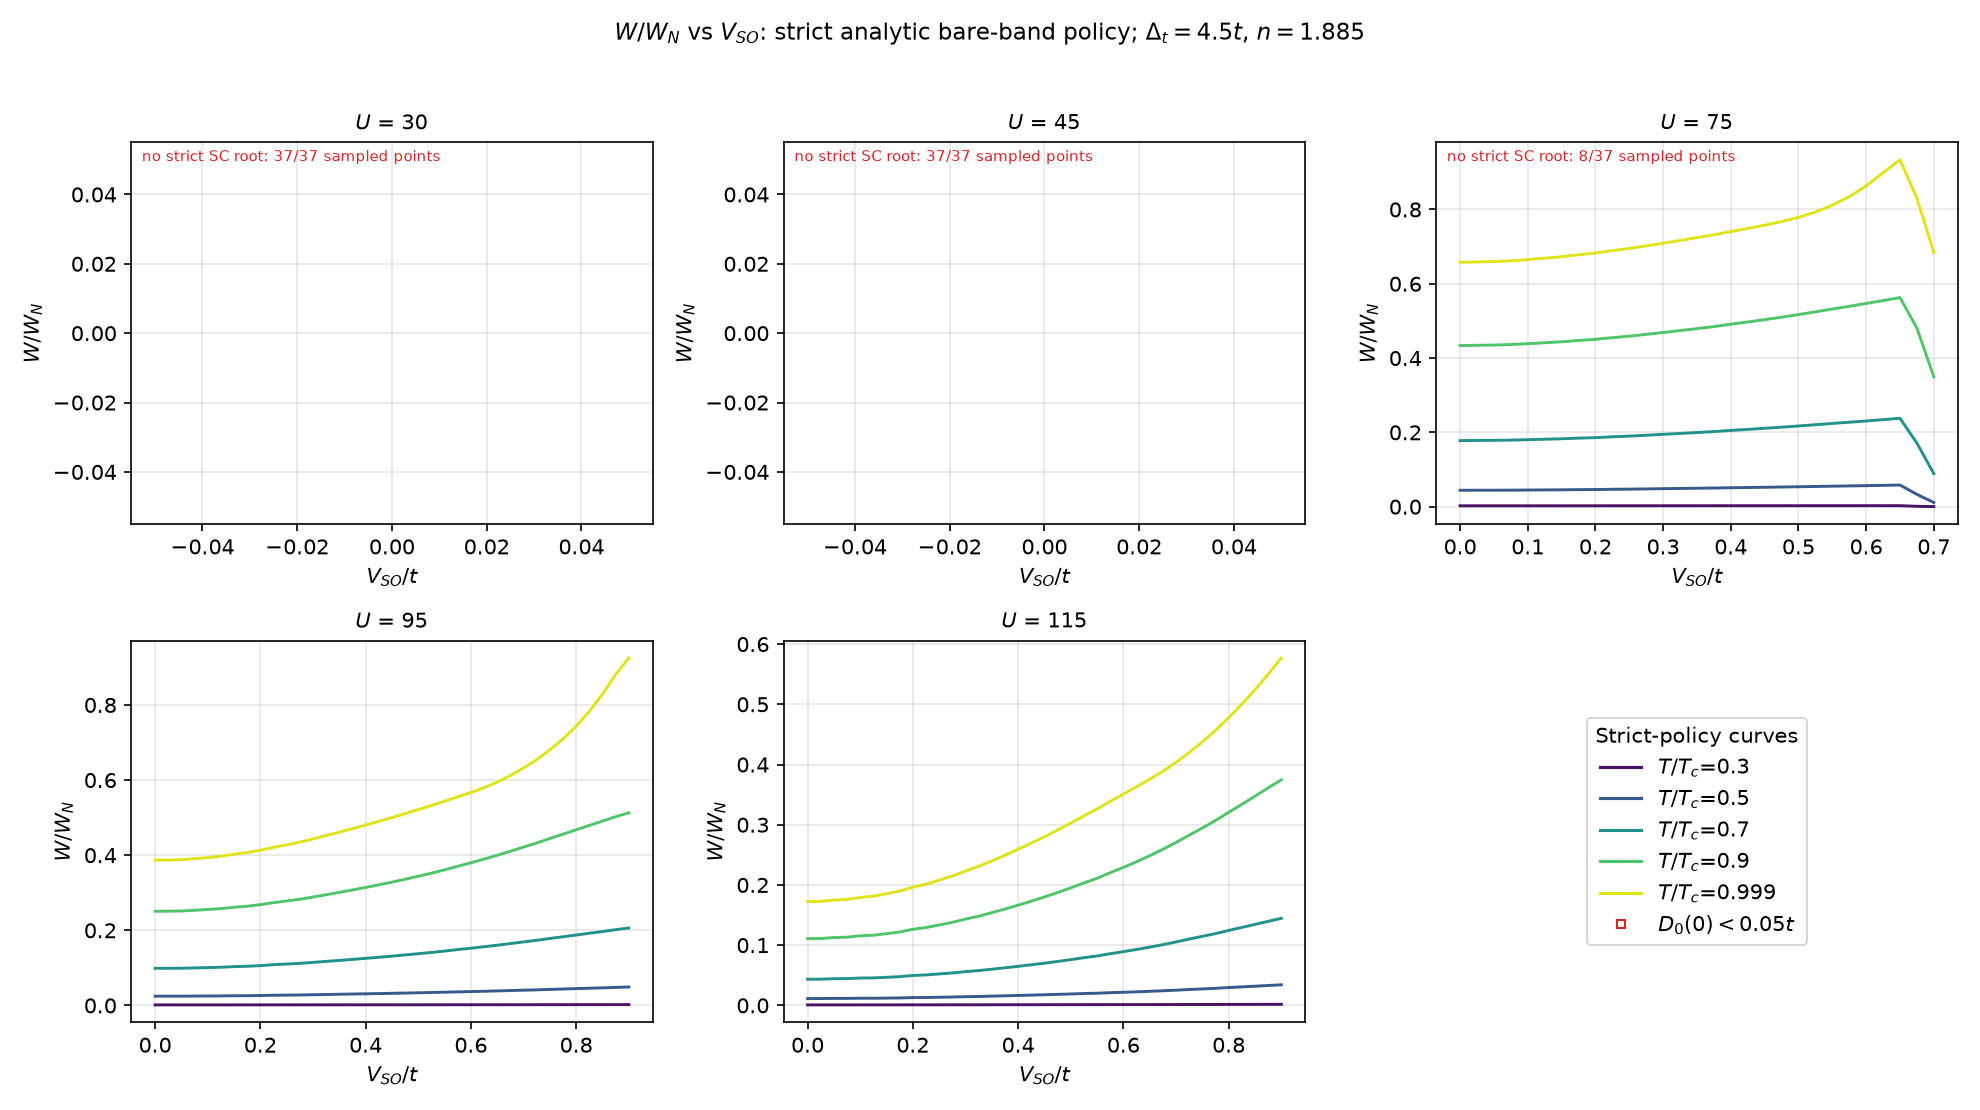
\includegraphics[width=\linewidth]{strict_policy/WWN_vs_VSO_families_U.png}
 \caption{Strict-window $W/W_N$ versus $V_{\mathrm{SO}}/t$ for the interaction families and temperature fractions marked in the panels. The displayed SOC trends are conditional on the shared constant matrix element and supplied gap/$T_c$ inputs; missing-root samples are gaps, not zeros. This scan complements the strict $U$-family figure and does not establish a universal SOC enhancement or suppression.}
 \label{fig:strict-soc}
\end{figure}

\subsection{Corrected legacy parameter families}

The next two composites retain figure families from the corrected first-paper calculations. They are included to connect the present draft to those parameter scans, but they use the archived relaxed-window roots rather than the regenerated strict-policy family data. Treat them as supplemental comparisons, not as replacements for the strict-window results above. In the $\Delta_t$ scan, the $\Delta_t=4.5t$ relaxed root has its zero-temperature chemical potential outside the bare-band interval; that curve is diagnostic under the stated professor-guided acceptance rule. This qualification does not assert that every relaxed root in every setting is generally unphysical.

\begin{figure}[t]
 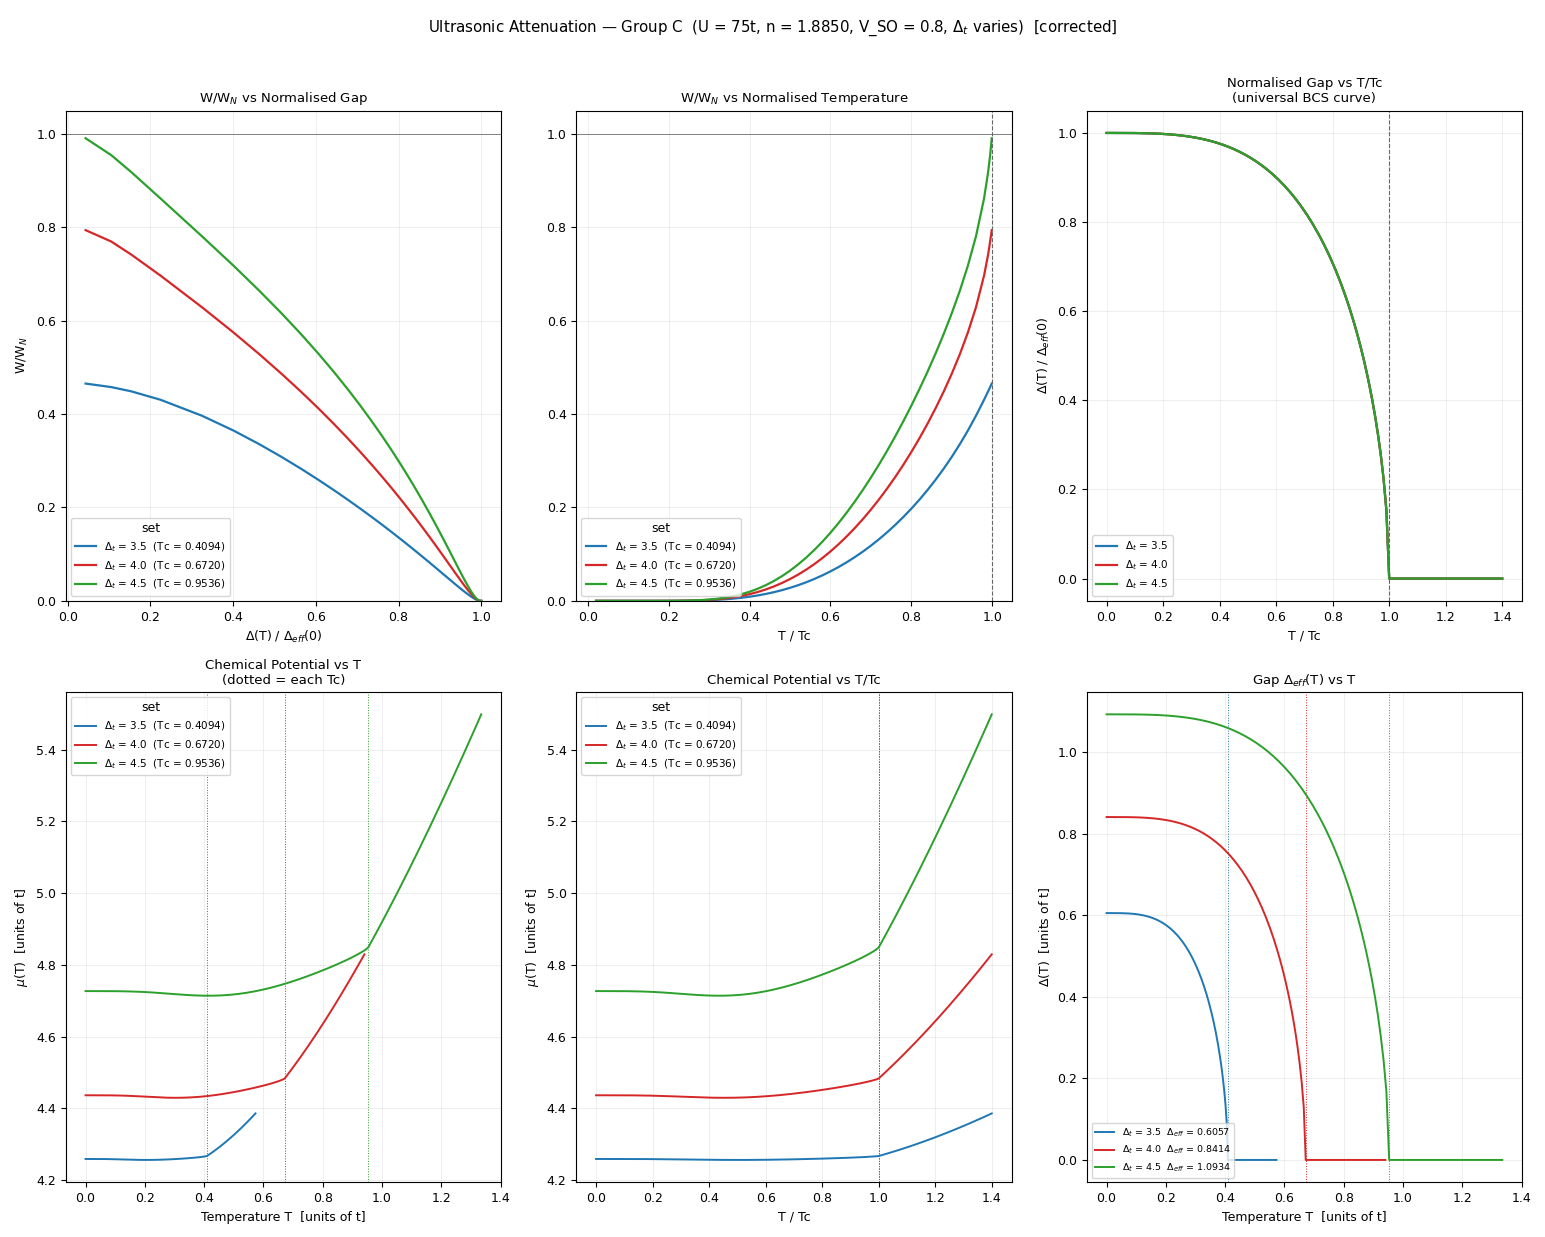
\includegraphics[width=\linewidth]{W_WN_groups_Dt_scan.png}
 \caption{Corrected Group-C composite from the first-paper figure set: $U=75t$, $n=1.885$, $V_{\mathrm{SO}}=0.8t$, with $\Delta_t$ varied. The absorption panels use archived relaxed-window roots; in particular, the $\Delta_t=4.5t$ zero-temperature root is out of band and is diagnostic, not a strict-policy acceptance result. The remaining gap, chemical-potential, and fitted-gap panels provide parameter context and are not additional attenuation observables.}
 \label{fig:legacy-delta-scan}
\end{figure}

\begin{figure}[t]
 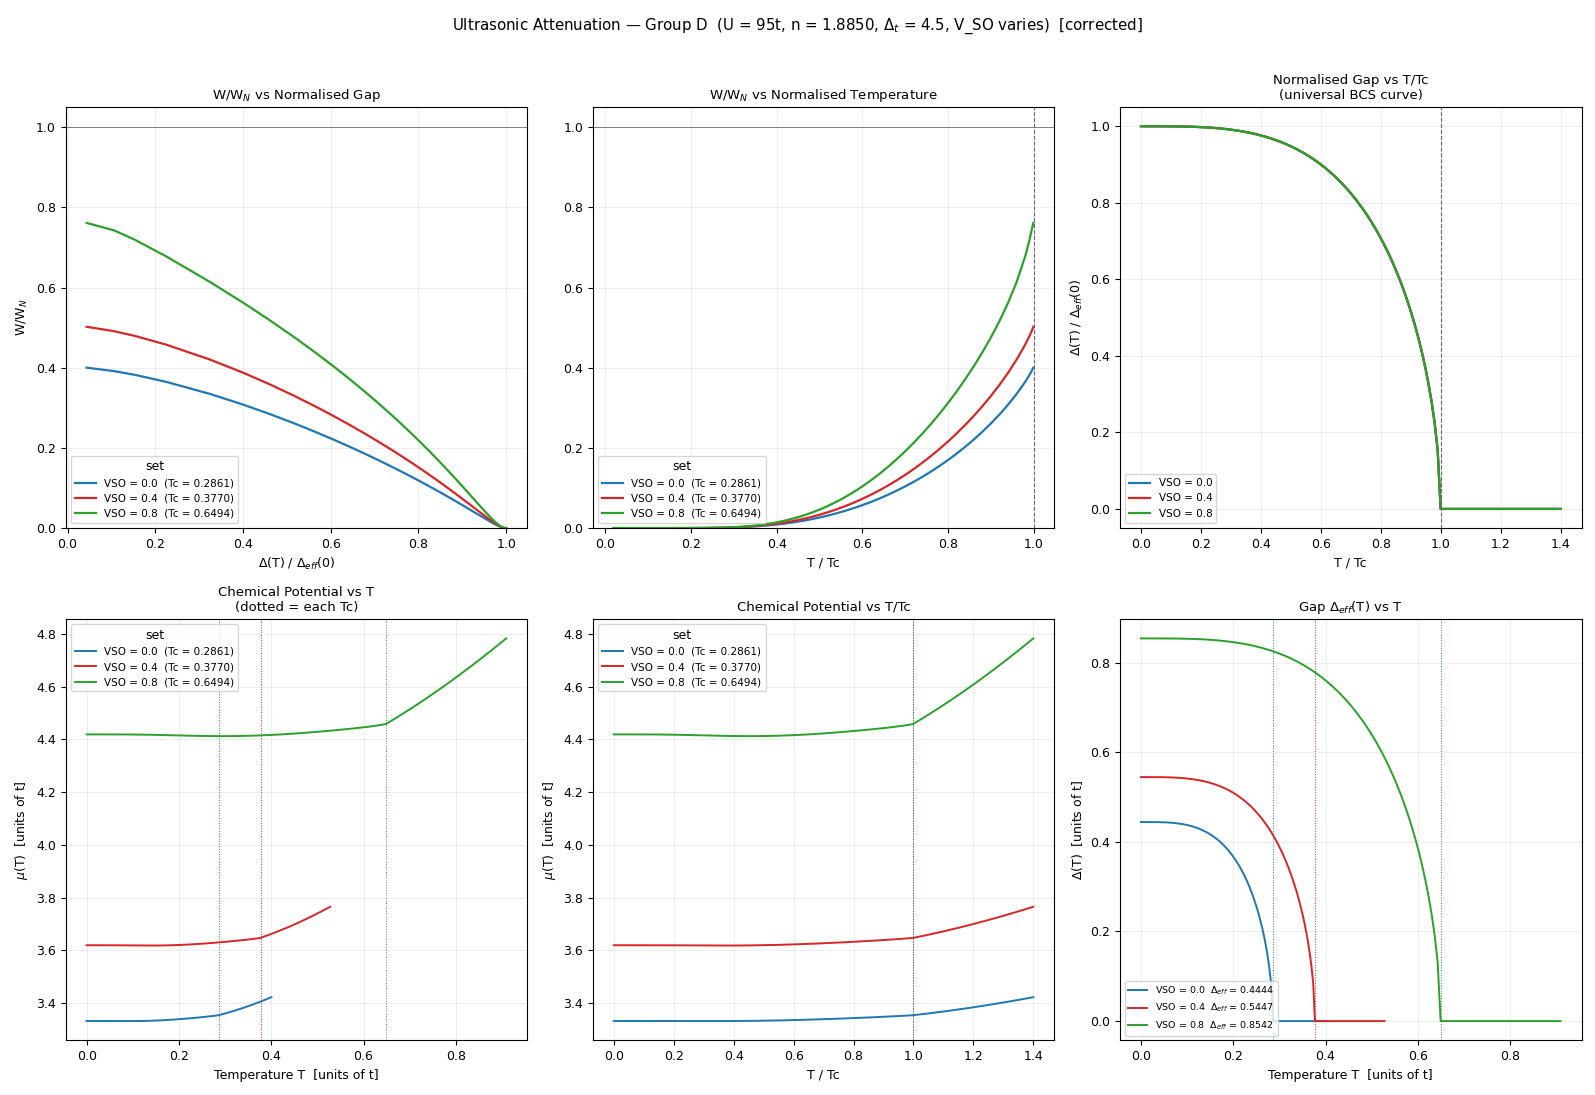
\includegraphics[width=\linewidth]{W_WN_groups_VSO_scan.png}
 \caption{Corrected Group-D composite from the first-paper figure set: $U=95t$, $n=1.885$, $\Delta_t=4.5t$, with $V_{\mathrm{SO}}$ varied. These curves use the archived relaxed-window family calculation and are retained as a supplemental comparison; they should not be conflated with the regenerated strict-policy SOC scan. The auxiliary panels show the fitted gap and chemical-potential state inputs.}
 \label{fig:legacy-vso-scan}
\end{figure}

\subsection{Sampled maxima and temperature envelopes}

We also analyze maxima from the existing sampled family data without a new response calculation. These scans use $\Delta_t=4.5t$, $n=1.885$, $\hbar\omega=0.7t$, $V_{\mathrm{SO}}/t=0,0.2,0.4,0.6,0.8$, and the stored $U=15t$--$150t$ grid at $0.5t$ spacing. For each policy, SOC, and sampled temperature fraction, the temperature-specific maximum is the largest finite $W/W_N$ on that grid; no interpolation or smoothing is used. The pointwise envelope instead takes the largest value over the five sampled temperatures at each sampled $U$. These are distinct operations, neither a continuous-domain optimization nor a free-energy stability test. The strict-only peak analysis is primary; relaxed-policy curves in the envelope are visibly separated and remain diagnostic.

\begin{figure}[t]
 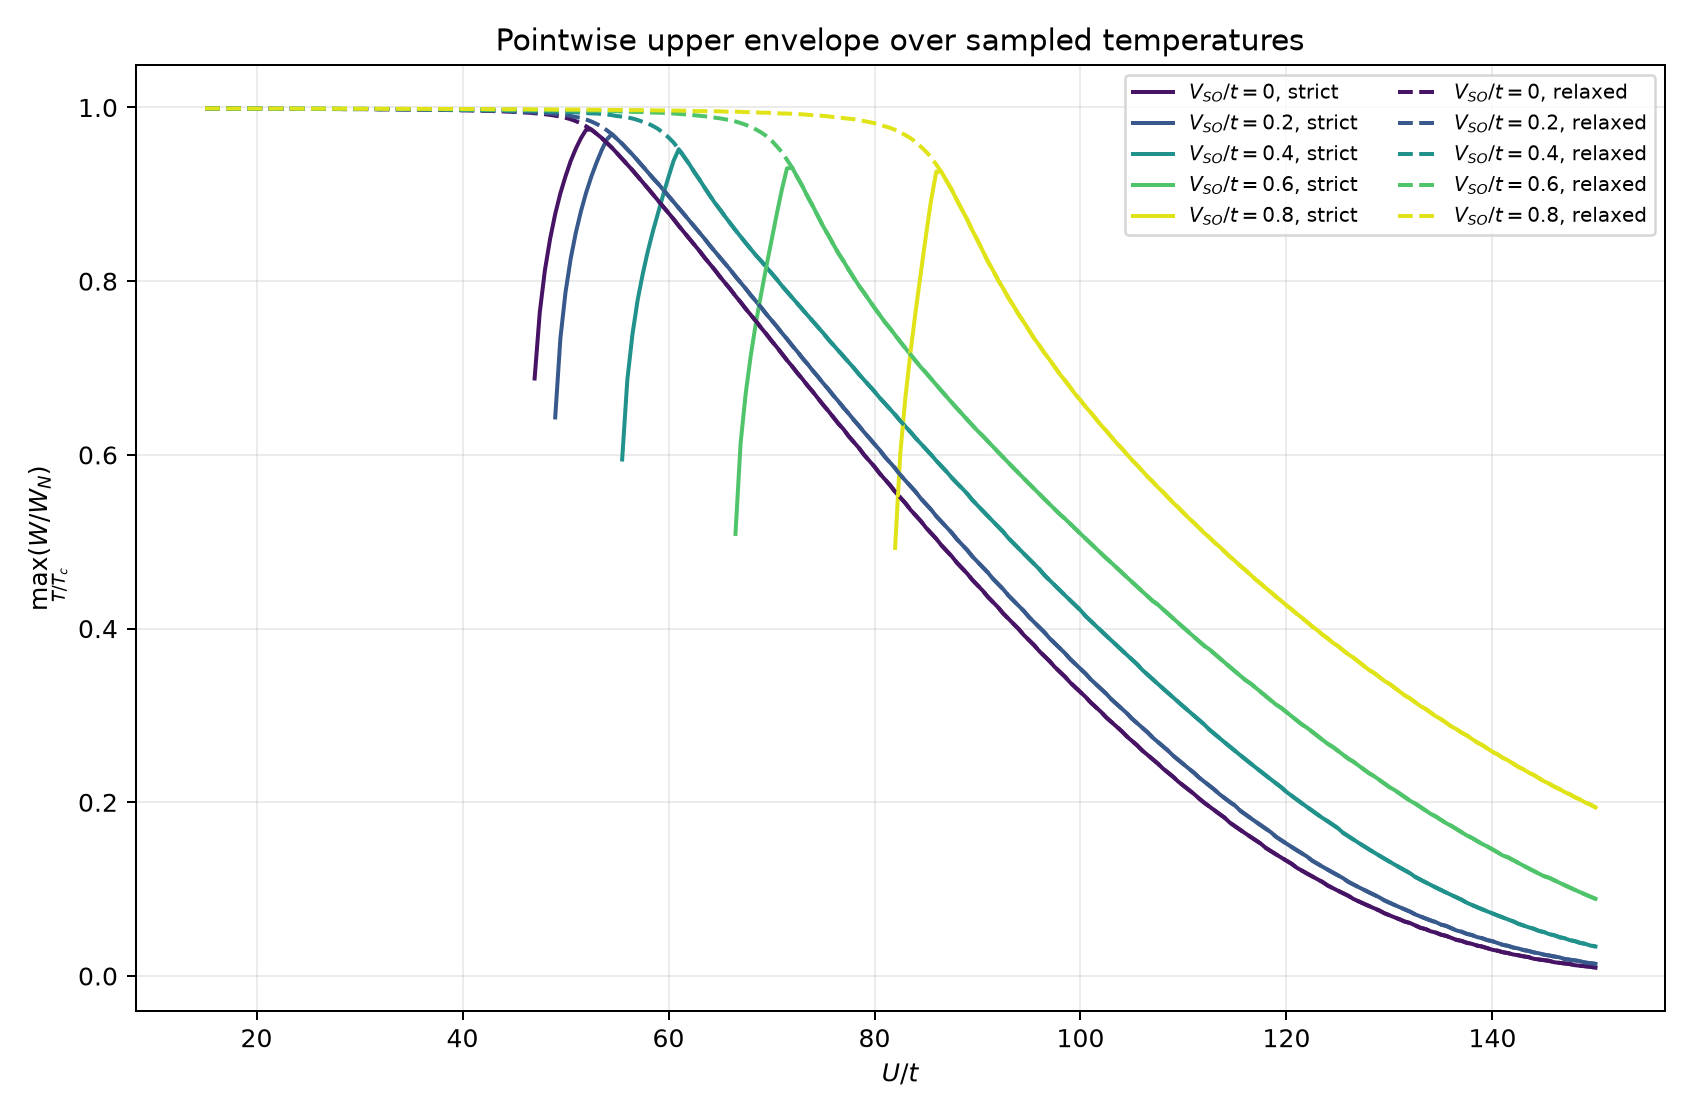
\includegraphics[width=\linewidth]{temperature_envelope_max_vs_U.png}
 \caption{Pointwise upper envelope of $W/W_N$ over the five sampled temperatures versus $U/t$, evaluated separately for each SOC and policy on the existing grid. Solid curves are strict-window results and are primary; dashed curves are relaxed-window diagnostics. At every $U$, the plotted value is the maximum among the available sampled temperatures, not an interpolated or continuous-temperature maximum. Relaxed roots are not substituted for missing strict values.}
 \label{fig:temperature-envelope}
\end{figure}

\begin{figure}[t]
 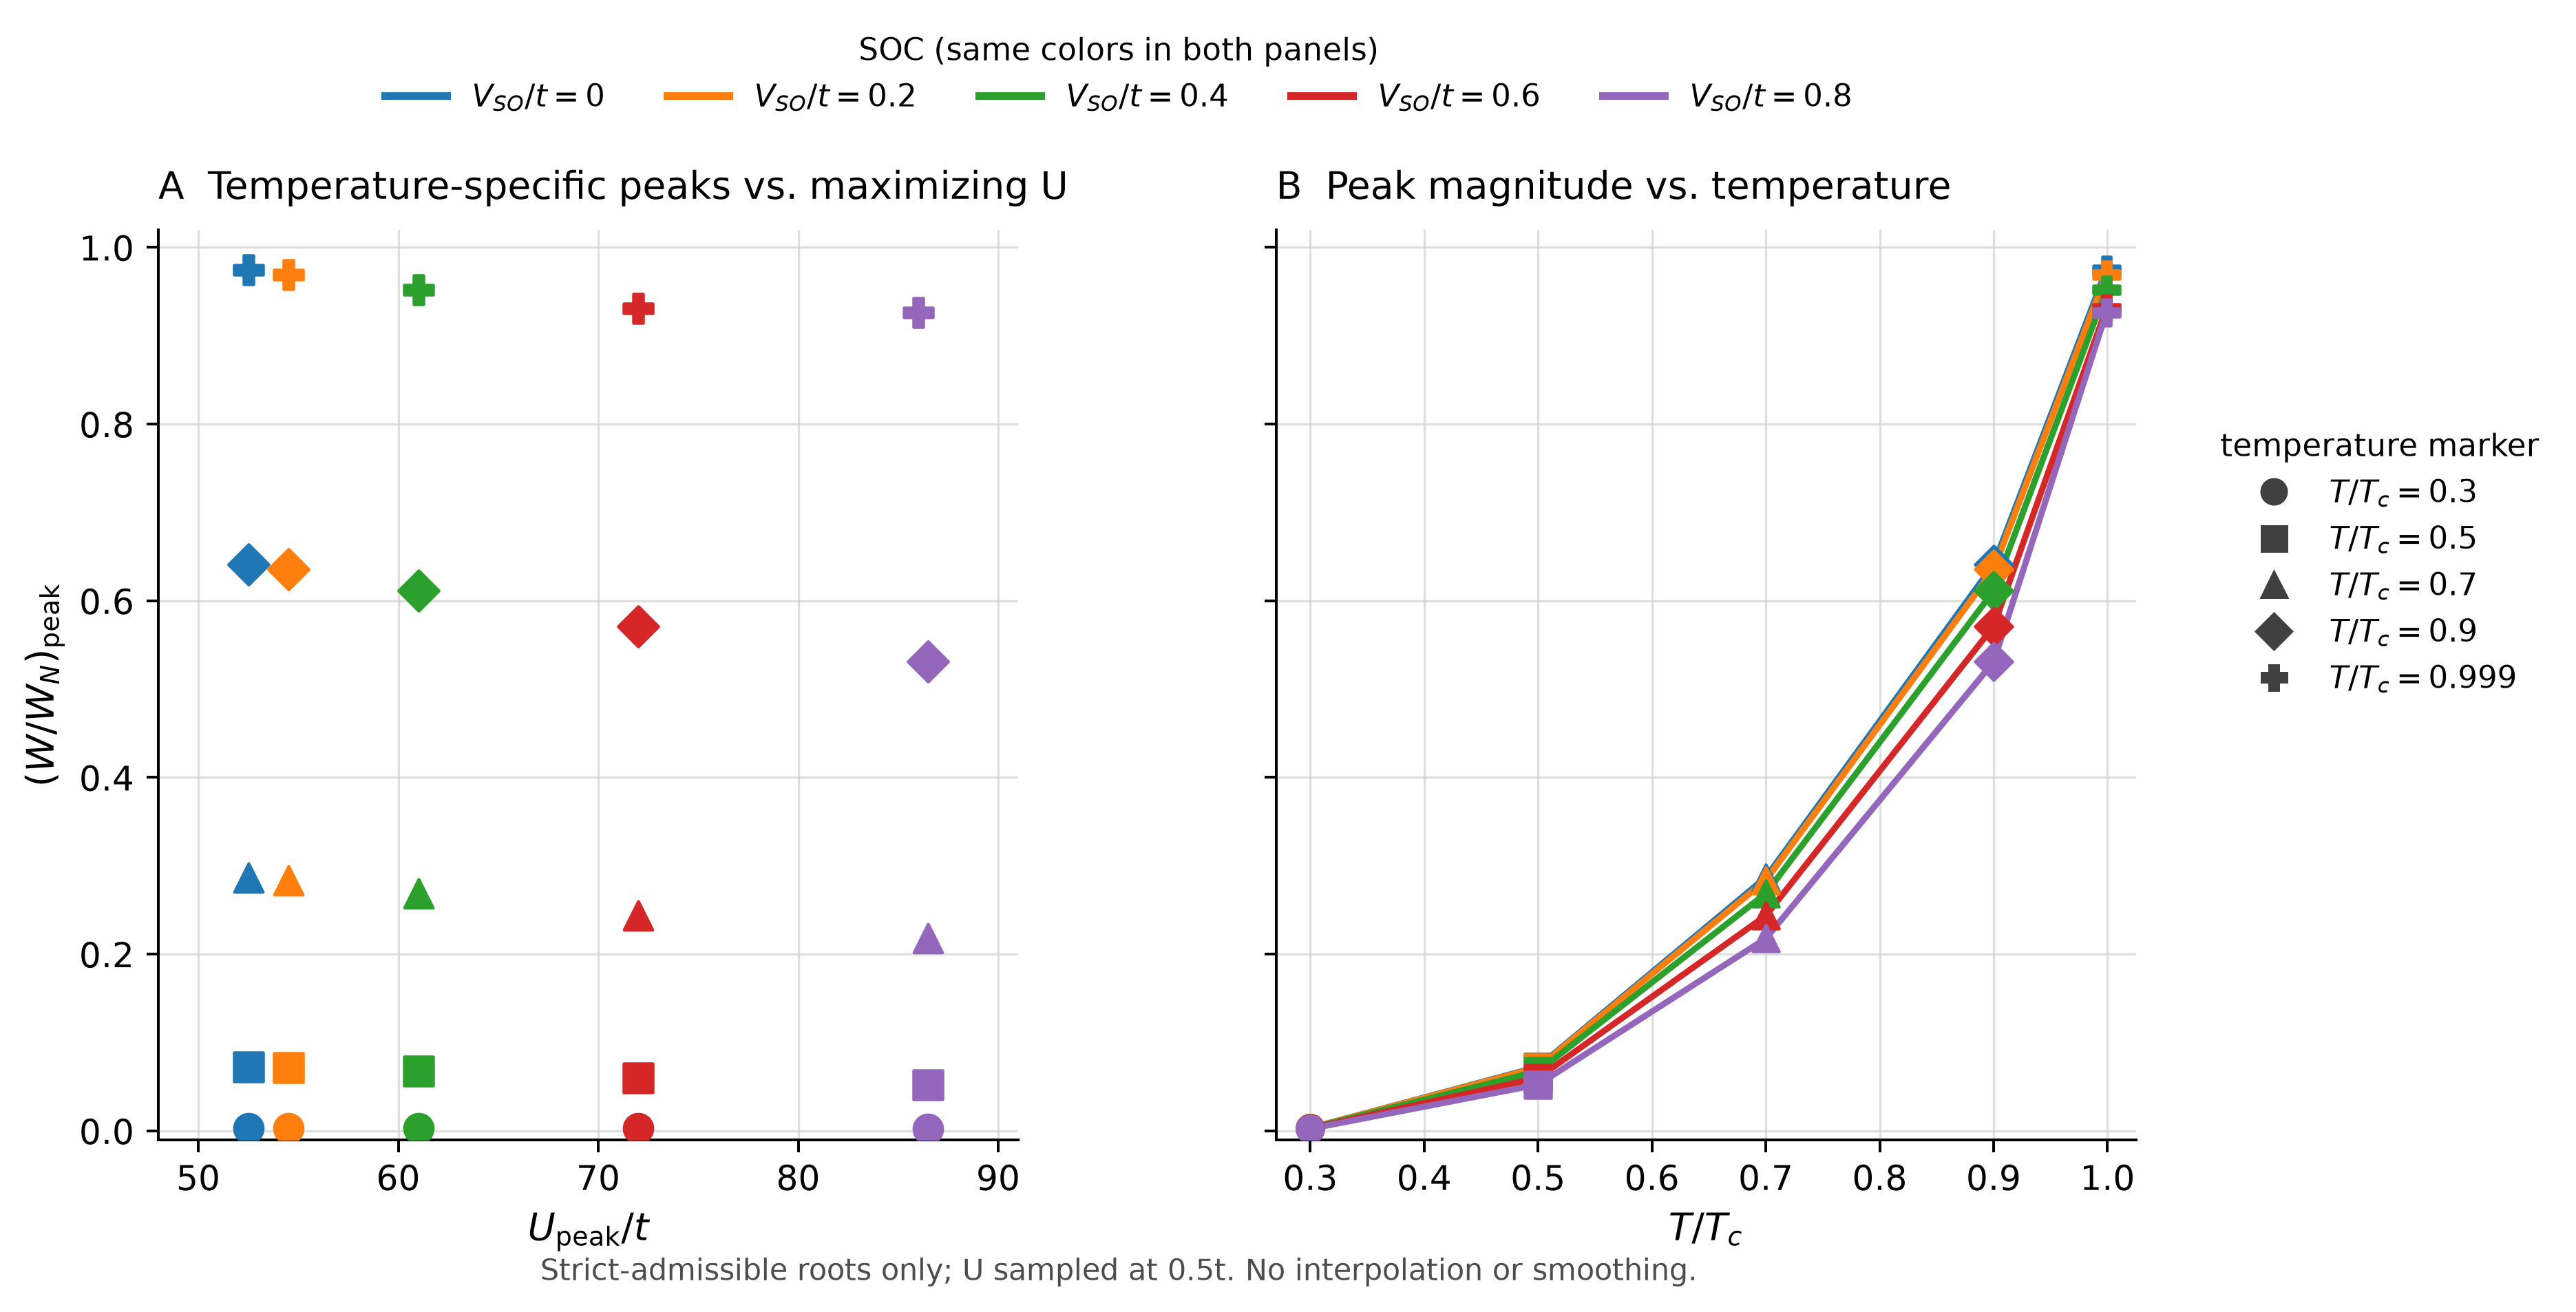
\includegraphics[width=\linewidth]{temperature_peak_analysis_two_panel.png}
 \caption{Strict-only sampled peak analysis. Panel A plots each temperature curve's exact sampled maximum as $(U_{\mathrm{peak}}/t,(W/W_N)_{\mathrm{peak}})$, with color denoting SOC and marker shape denoting $T/T_c$; points are neither jittered nor connected, and the maximizing $U$ values are retained exactly. Panel B shows those same peak magnitudes against the five sampled temperatures. All 25 maxima lie inside their strict-admissible $U$ intervals; this finite-grid analysis does not interpolate between samples.}
 \label{fig:strict-temperature-peaks}
\end{figure}

For the strict-only peak data, the sampled maximizing interaction shifts upward with SOC: from $U_{\mathrm{peak}}/t=52.5$ at $V_{\mathrm{SO}}/t=0$ to $86.5$ at $V_{\mathrm{SO}}/t=0.8$ for $T/T_c=0.3$--$0.9$ (the $T/T_c=0.999$ maximum at the latter SOC occurs at $86.0$). At $T/T_c=0.999$, the sampled peak height decreases from $0.9746$ at zero SOC to $0.9262$ at $V_{\mathrm{SO}}/t=0.8$. These are exact maxima on the stored $0.5t$ grid, not estimates of continuous extrema; the underlying family model uses the repository's fitted gap shape and does not rank multiple in-band roots by free energy.

The branch-decomposition figure separates the energy-inversion branches and compares the spectral threshold $2E_{\min}$ with the commonly plotted effective-gap scale. This is a property of the adopted quasiparticle spectrum; it does not replace a finite-$q$ response calculation.

\begin{figure}[t]
 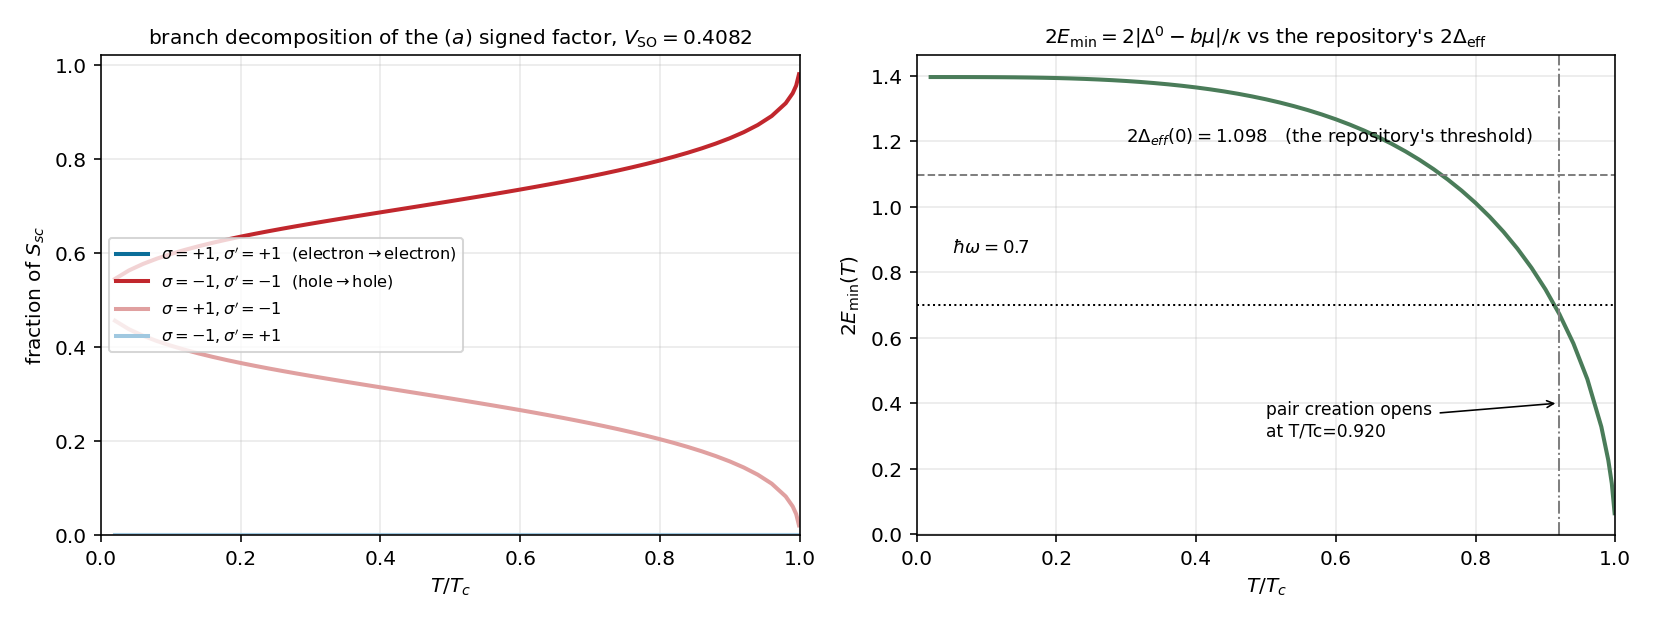
\includegraphics[width=\linewidth]{branch_decomposition.png}
 \caption{Branch-resolved decomposition of the constant-vertex scattering model and the model threshold $2E_{\min}=\hbar\omega$ for the displayed parameter set. The branch index $\sigma$ labels the two roots of $E(\epsilon)$, not Rashba helicity. The comparison with $2\Delta_{\mathrm{eff}}$ illustrates that the effective-gap scale is not the exact spectral threshold when the gap depends on band energy. This figure is a model diagnostic, not a finite-$q$ acoustic prediction.}
 \label{fig:branches-threshold}
\end{figure}

The main energy-space calculation is checked against an independent lattice-energy-binning implementation and against the isotropic $s$-wave, flat-DOS, $\omega\to0$ limit. The latter reproduces the attenuation ratio $2f(\Delta(T))$ in the regime of the Levy benchmark~\cite{Levy}. These checks test the coherence-factor algebra, density-of-states normalization, and numerical integration under the model assumptions. They do not test the missing phonon vertex or the momentum selection of a real acoustic mode.

\begin{figure}[t]
 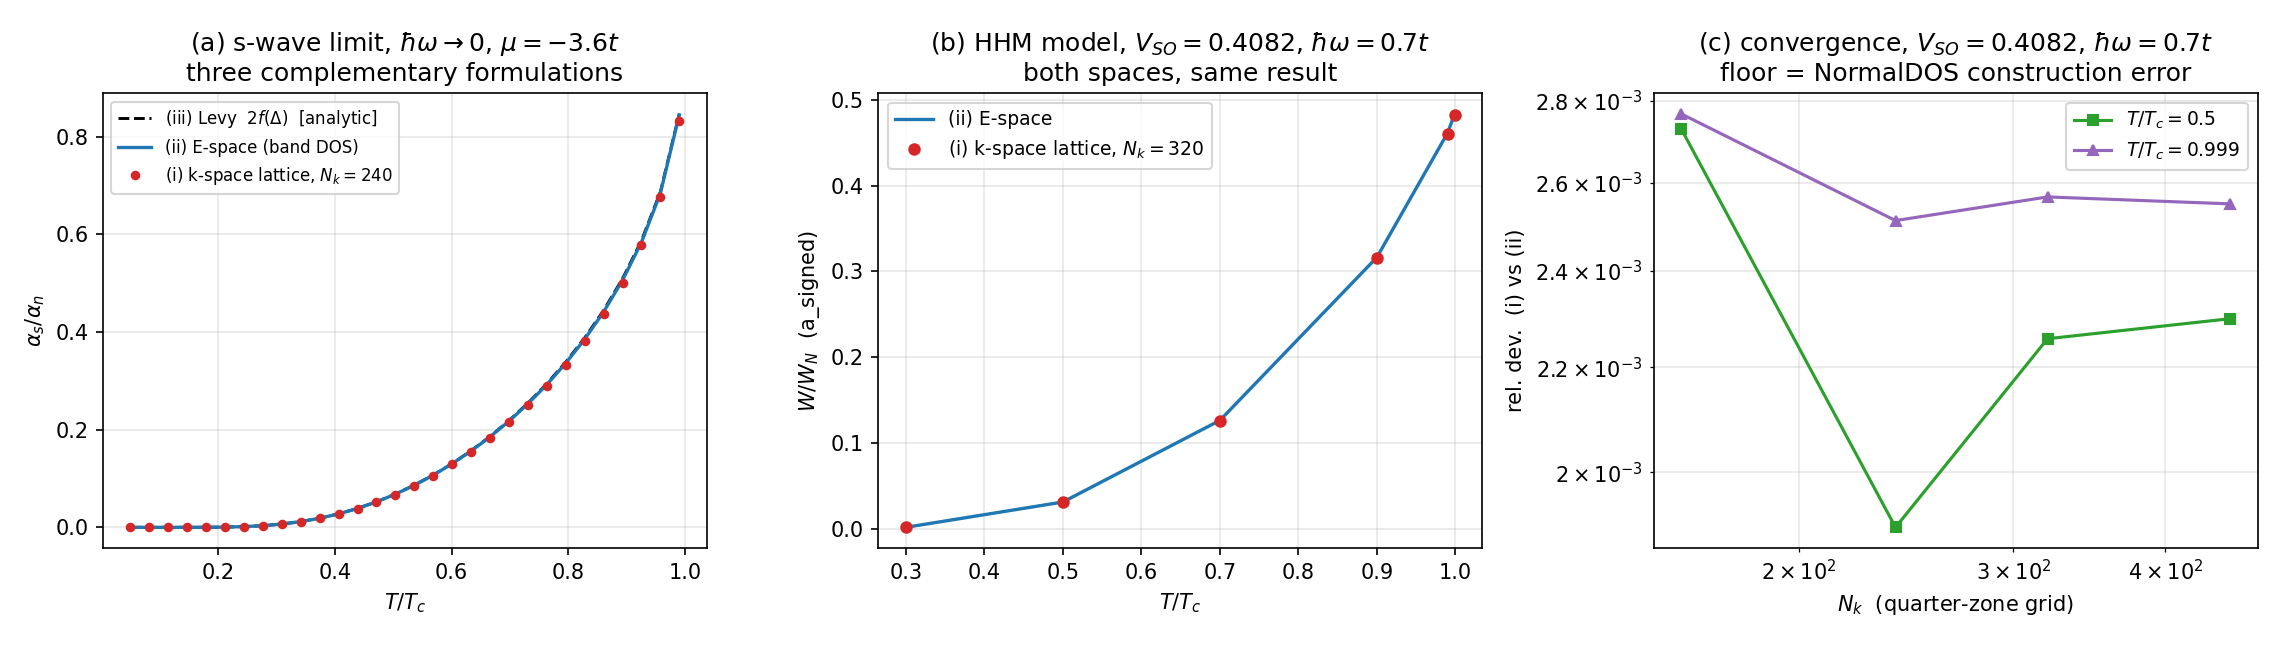
\includegraphics[width=\linewidth]{dual_space_k_vs_energy.png}
 \caption{Numerical cross-check of the lattice-energy-binning and energy-space formulations and a separate $s$-wave benchmark. Agreement tests the implementation of the unrestricted constant-vertex integral; it is not independent evidence for the microscopic acoustic coupling.}
 \label{fig:numerical-crosscheck}
\end{figure}

\section{Vertex sensitivity and limitations}

The production integral's total-DOS product effectively assigns the same matrix element to every helicity pair. A separate code diagnostic compares this isotropic all-helicity prescription with a same-helicity prescription motivated by the $q\to0$ scalar-density overlap. The difference is visible in the vertex-sensitivity diagnostic. The latter is not a full finite-$q$ calculation: it filters helicity labels but still lacks the $\bm k,\bm q$-dependent matrix element and the acoustic dispersion.

\begin{figure}[t]
 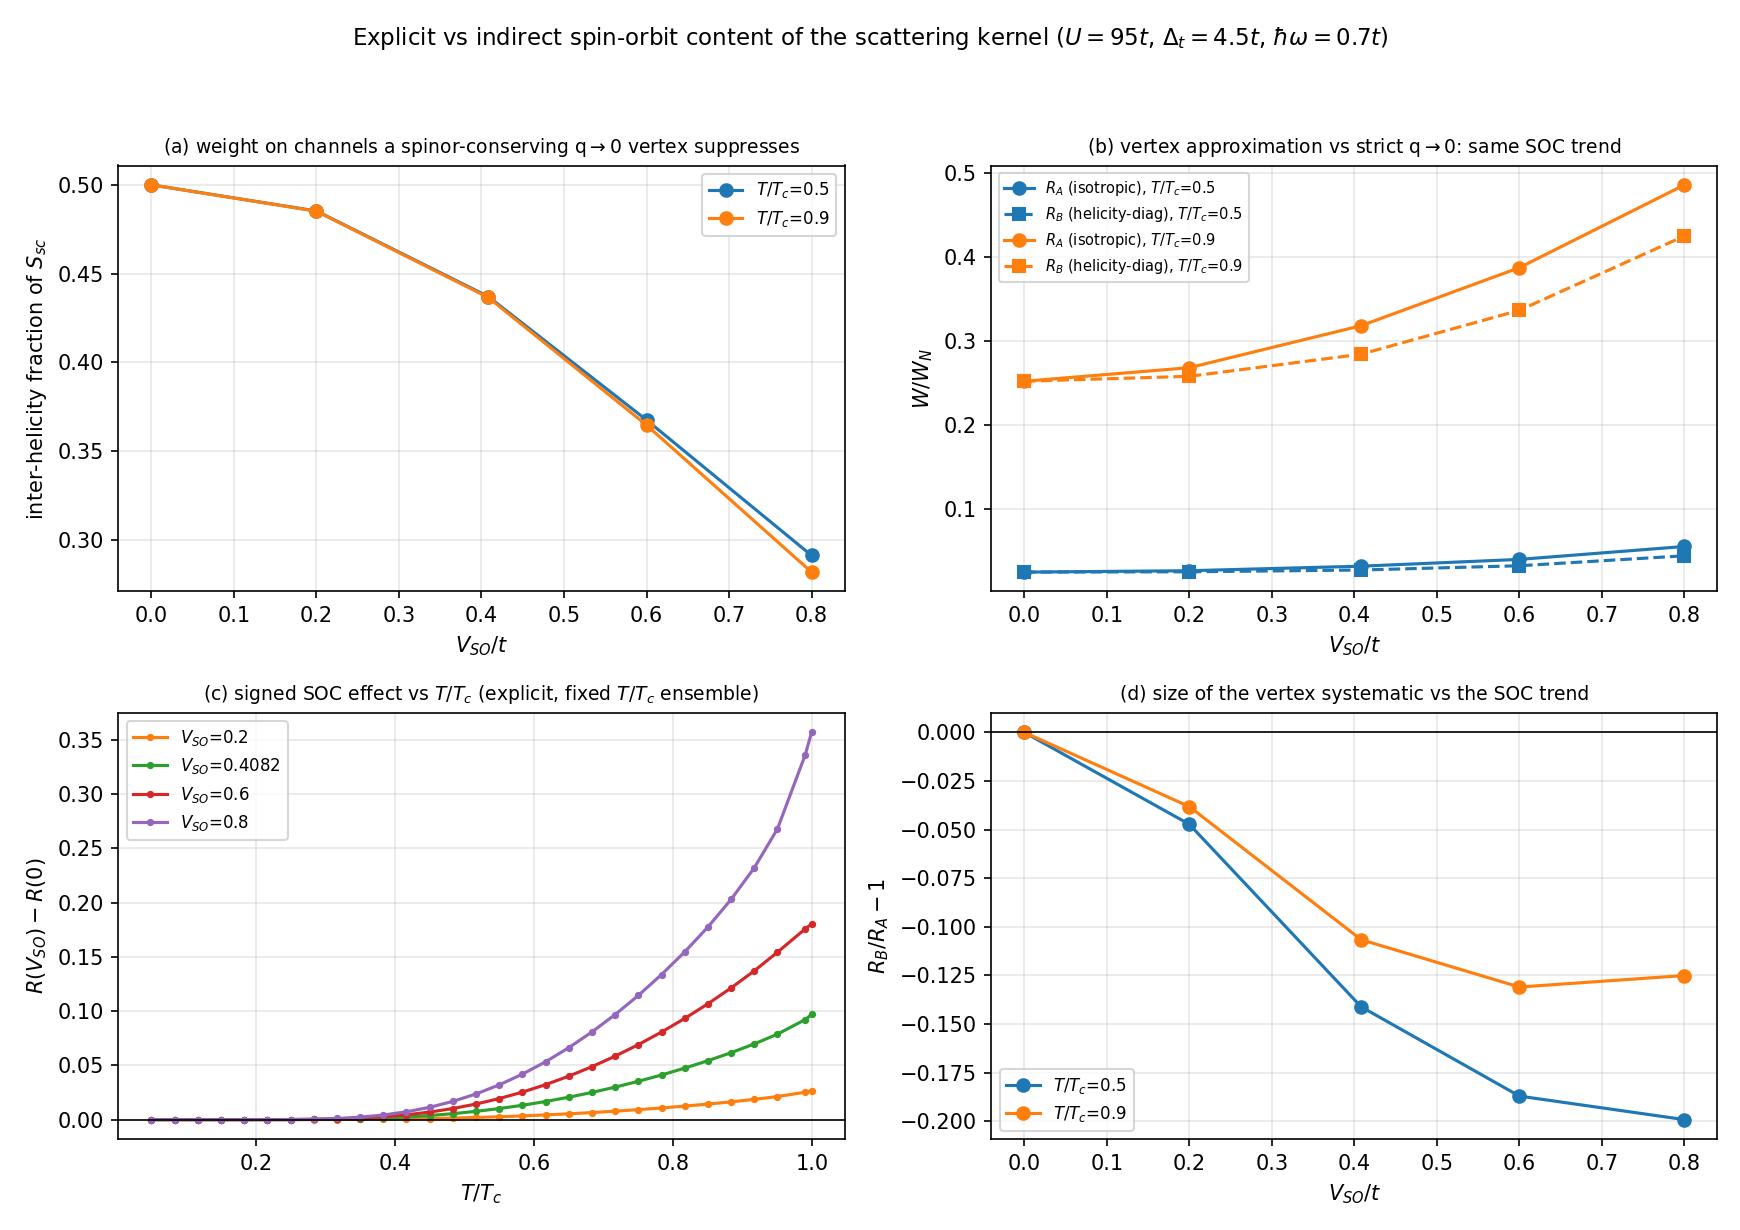
\includegraphics[width=\linewidth]{soc_explicit_vertex.png}
 \caption{Repository diagnostic comparing all-helicity and same-helicity constant-vertex prescriptions. It illustrates sensitivity to vertex selection; it is not a momentum-conserving or finite-$q$ acoustic calculation and should not be used as a corrected physical prediction.}
 \label{fig:vertex-sensitivity}
\end{figure}

Several further ingredients are needed for a physical ultrasonic attenuation calculation: (i) a microscopic or measured strain vertex, including ordinary and correlated hopping and any Rashba modulation; (ii) phonon branch, polarization, mass density, and $v_s$; (iii) fixed-$q$ BdG matrix elements with $\bm k'=\bm k+\bm q+\bm G$; and (iv) an assessment of charge screening, collective phase response, disorder, and conserving vertex corrections. At exactly $q=0$, the total-density operator is conserved in the number-conserving theory, so a finite-frequency bare density response must be treated with the appropriate order of limits and gauge-restoring response corrections. None of these quantities is determined by the current electronic parameter set.

\section{Conclusion}

We have written the corrected energy-space expression for the quasiparticle-scattering component of a Rashba-correlated-hopping superconducting model. The signed Case-I coherence factor, branch-resolved density of states, and normal reference are consistent within the stated mean-field and constant-matrix-element assumptions. The repository's finite-grid and limiting-case checks support the numerical implementation of that model.

The calculation does not establish a microscopic acoustic coupling. In particular, a constant all-to-all matrix element is not generally equivalent to a finite-$q$ phonon perturbation with momentum conservation, and the HHM Hamiltonian supplies none of the required strain derivatives. Consequently, the figures document model-dependent normalized absorption, not a validated material-specific ultrasonic attenuation or a universal SOC trend. A finite-$q$ calculation should follow only after the phonon mode and electron--ion vertex have been supplied or derived.

\begin{acknowledgments}
The authors thank colleagues for discussions. [Please replace this placeholder with the appropriate acknowledgments and funding information.]
\end{acknowledgments}

\appendix
\section{Generic finite-$q$ BdG response}

For a specified acoustic perturbation, the positive-energy quasiparticle-scattering contribution has the structure
\begin{align}
 P_{\mathrm{sc}}(\bm q,\lambda)={2\pi\over\hbar}(\hbar\omega_{\bm q\lambda})
 \sum_{\bm k,m,n}|M_{nm}(\bm k,\bm q,\lambda)|^2
 &[f(E_{m\bm k})-f(E_{n,\bm{k+q}})]\\[-2pt]
 &\times\delta(E_{n,\bm{k+q}}-E_{m\bm k}-\hbar\omega_{\bm q\lambda}),
 \label{eq:finiteq-sc}
\end{align}
with $M$ from Eq.~(\ref{eq:bdg-matrix-element}) and crystal momenta folded modulo reciprocal vectors. Pair creation has a thermal factor $1-f(E_{m\bm k})-f(E_{n,\bm{q-k}})$ and energy delta $\delta(E_{m\bm k}+E_{n,\bm{q-k}}-\hbar\omega_{\bm q\lambda})$. The equations specify the kinematics and matrix-element structure only; the normalizations and numerical response require the missing microscopic vertex and mode data.

The scalar Rashba overlap in Eq.~(\ref{eq:helicity-overlap}) follows from the helicity projectors $P_s(\bm k)=[1+s\hat{\bm g}_{\bm k}\cdot\bm\sigma]/2$. For a non-scalar strain vertex, the spin matrix elements must be evaluated with that vertex rather than multiplied by this scalar overlap as an independent factor.

\bibliographystyle{apsrev4-2}
\bibliography{draft_references}

\end{document}
